\documentclass{article}

\usepackage[margin = 1in]{geometry}

\usepackage{graphicx, amsmath}
\graphicspath{ {./images/} }

\title{Ch. 7 Solutions}
\author{Principles of Microeconomics}
\date{\today}

\begin{document}

\maketitle

\section*{Quick Quiz}

\begin{enumerate}

\item (b) --
	\begin{align*}
	CS_A &= 12 - 6 = 6 \\
	CS_B &= 8 - 6 = 2 \\
	CS_C &= 0 \\
	CS_{mkt} &= 6 + 2 = 8
	\end{align*}

\item (b) --
	\begin{align*}
	CS_A &= 12 - 3 = 9 \\
	CS_B &= 8 - 3 = 5 \\
	CS_C &= 4 - 3 = 1 \\
	CS_{mkt} &= 9 + 5 + 1 = 15 \\
	\Delta CS_{mkt} &= 15 - 8 = 7
	\end{align*}
	
\item (d) --
	\begin{center}
	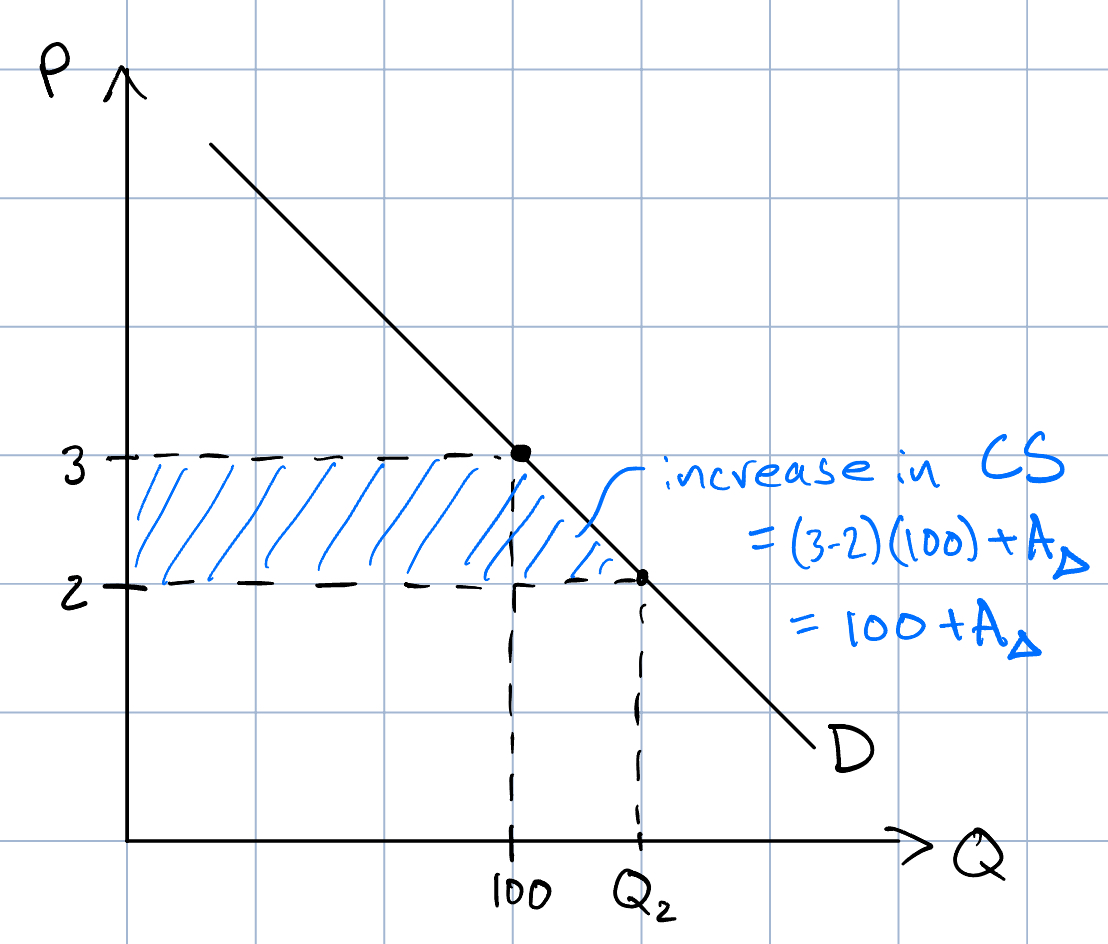
\includegraphics[width = 0.3\textwidth]{ch7_qq3}
	\end{center}
	
\item (c) --
	\begin{align*}
	PS_{Diego} &= 0 \text{ (because he doesn't take the job)} \\
	PS_{Emi} &= 300 - 200 = 100 \\
	PS_{Finn} &= 300 - 100 = 200 \\
	PS_{Mkt} &= 0 + 100 + 200 = 300
	\end{align*}
	
\item (b) -- Gavin's PS rises by \$100 because $PS = P - Cost$ and $P$ increased by 100. Hector's cost is higher than \$300 but lower than \$400 because he didn't work when the price was \$300 but he does when the price is \$400. That means his PS is 400 minus a number between 300 and 400, so his PS is between 0 and 100. Therefore, producer surplus increases 100 plus something between 0 and 100. 

\item (c) --
	\begin{center}
	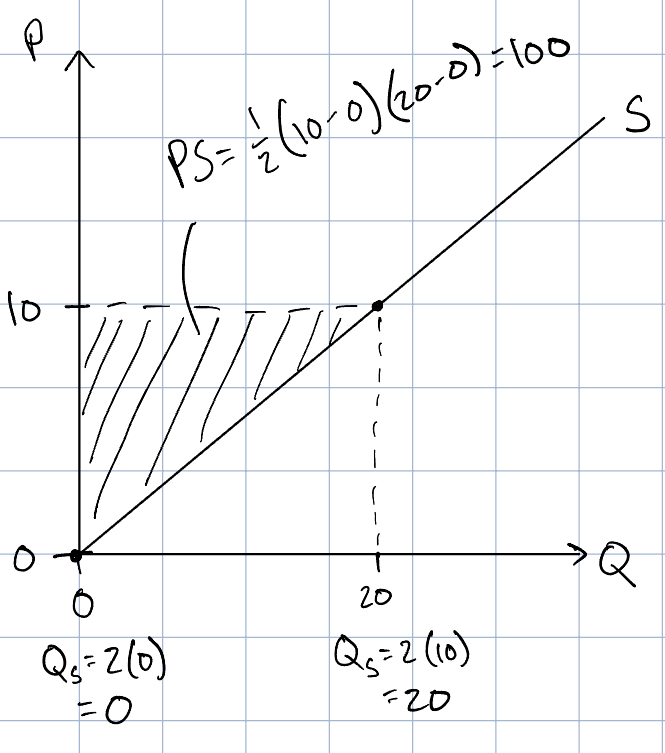
\includegraphics[width = 0.3\textwidth]{ch7_qq6}
	\end{center}
	
\item (a) --
	\begin{align*}
	CS &= WTP - P \\
	&= 300 - 200 \\
	&= 100 \\
	PS &= P - Cost \\
	&= 200 - 2(60) \\
	&= 80 \\
	CS - PS &= 100 - 80 \\
	&= 20
	\end{align*}
	
\item (c) -- By definition, an efficient outcome maximizes total surplus which is the sum of consumer surplus and producer surplus.

\item (b) -- At equilibrium, buyers and sellers are represented by the segments of the demand and supply curves to the left of equilibrium. Since those are the highest and lowest segments of the demand and supply curves respectively, the buyers and sellers are those with the highest willingnesses to pay and lowest costs.

	\begin{center}
	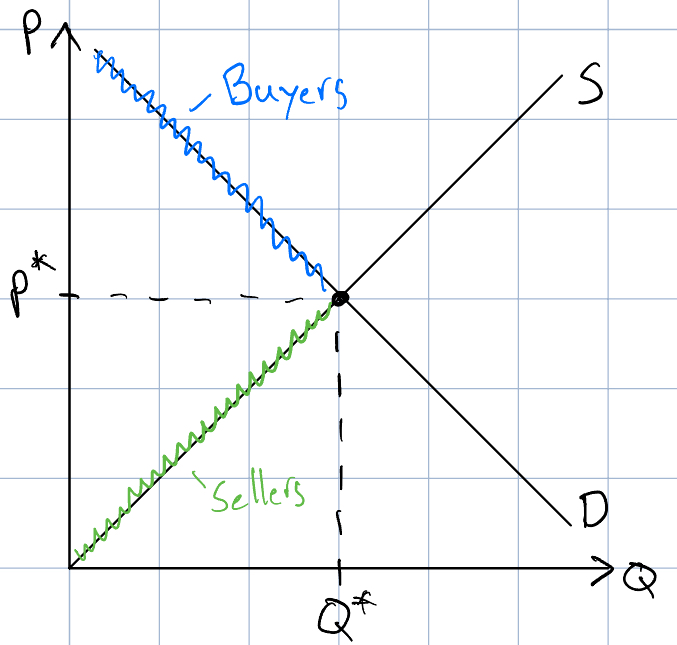
\includegraphics[width = 0.3\textwidth]{ch7_qq7}
	\end{center}
	
\item (c) -- At a quantity to the right of equilibrium, the demand curve is below the supply curve. That mean's the marginal buyer's willingness to pay is less than the marginal seller's cost of production.

\end{enumerate}

\section*{Questions for Review}

\begin{enumerate}

\item Willingness to pay is used to calculate an individual's consumer surplus: $CS = WTP - P$. The height of the demand curve measures willingness to pay. Consumer surplus in a market is the area beneath the demand curve and above price.

\item Cost is used to calculate a firm's producer surplus: $PS = P - Cost$. The height of the supply curve measures cost. Producer surplus in a market is the area beneath price and above the supply curve.

\item \phantom{x}

	\begin{center}
	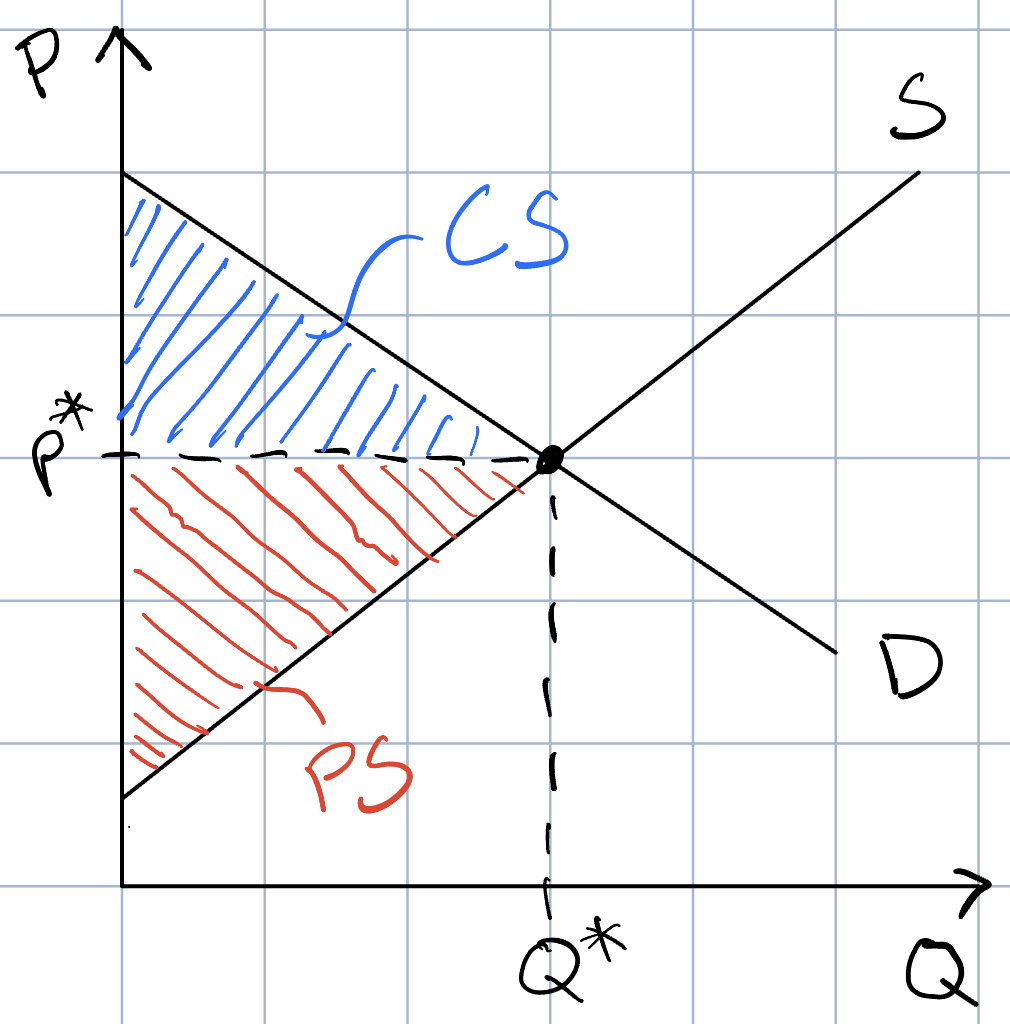
\includegraphics[width = 0.3\textwidth]{ch7_qfr3}
	\end{center}
	
\item An allocation of resources is efficient if it maximizes total surplus. In other words, an allocation of resources is efficient if it maximizes the benefit accruing to consumers plus the benefit accruing to producers of that resource.

\item Market power -- If a market isn't competitive, some buyers or sellers have market power. Market power gives them the ability to influence the price which can prevent the market from reaching its efficient equilibrium.

Externalities -- If a market has externalities (side effects that impact bystanders), buyers and sellers might not take those externalities into account when deciding how much to consume and produce. The market equilibrium might be inefficient because it doesn't account for the effect on bystanders. 

\end{enumerate}

\section*{Problems and Applications}

\begin{enumerate}

\item 

	\begin{enumerate}
	
	\item

		\begin{align*}
		CS &= WTP - P \\
		240 &= WTP - 360 \\
		600 &= WTP
		\end{align*}
		
	\item
		
		\begin{align*}
		CS &= 600 - 270 \\
		CS &= 330
		\end{align*}
		
	\item She wouldn't have bought an iPhone because \$750 is more than her willingness to pay. With no purchase, her consumer surplus would have been 0.
		
	\end{enumerate}
	
\item The freeze reduces the supply of lemons, so the supply curve shifts left. That increases the price and decreases the quantity of lemons sold, so consumer surplus decreases.

	\begin{center}
	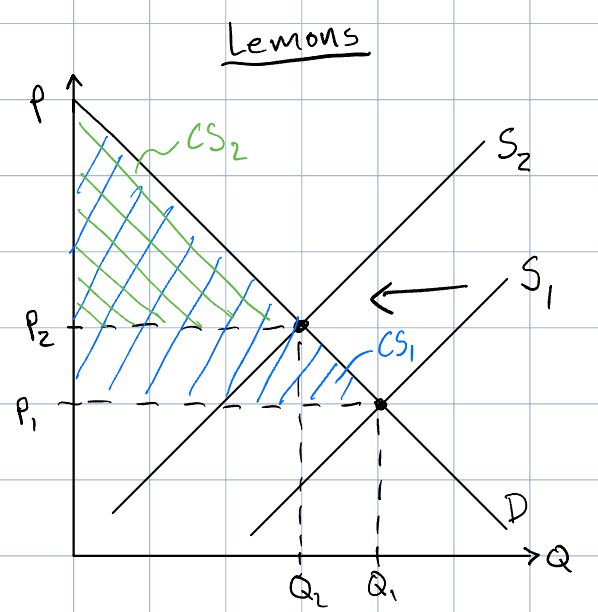
\includegraphics[width = 0.3\textwidth]{ch7_paa2_lemons}
	\end{center}
	
Lemons are an input to lemonade, so when the price of lemons increases, the supply of lemonade decreases. The supply curve for lemonade shifts left which increases the price and decreases the quantity of lemonade sold. As a result, consumer surplus goes down.

	\begin{center}
	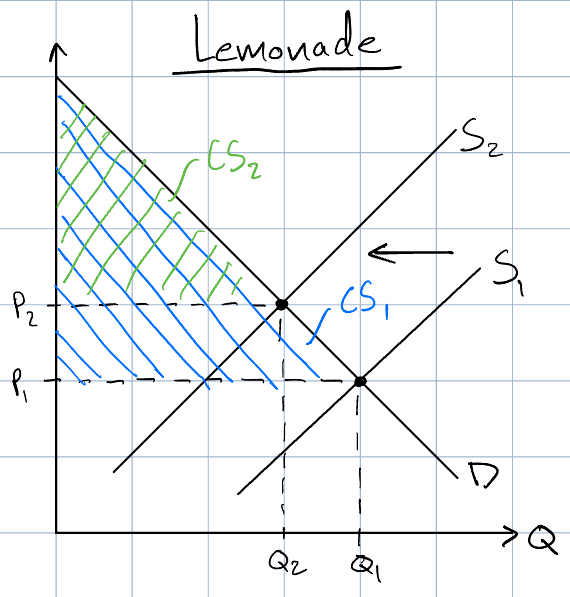
\includegraphics[width = 0.3\textwidth]{ch7_paa2_lemonade}
	\end{center}
	
\item When demand for French bread rises, the price rises. As a result, producer surplus increases.

	\begin{center}
	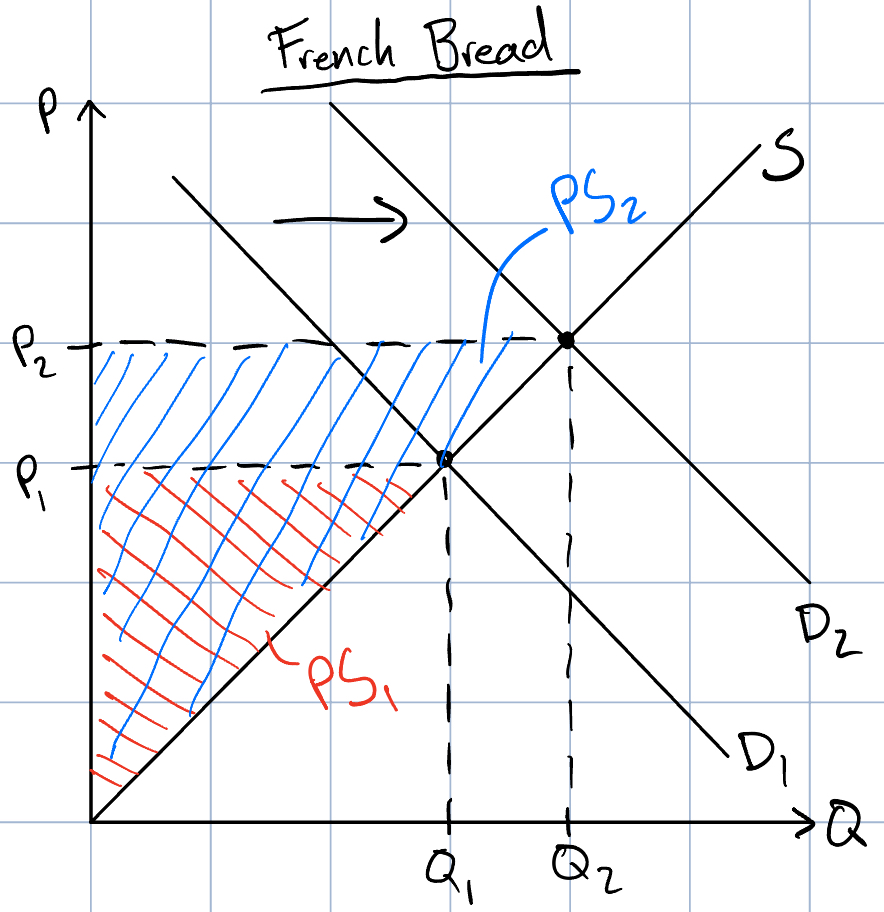
\includegraphics[width = 0.3\textwidth]{ch7_paa3_bread}
	\end{center}
	
	The quantity of french bread produced increases, so there are more buyers of flour. That increases demand for flour which increases the price. As a result, producer surplus increases.
	
	\begin{center}
	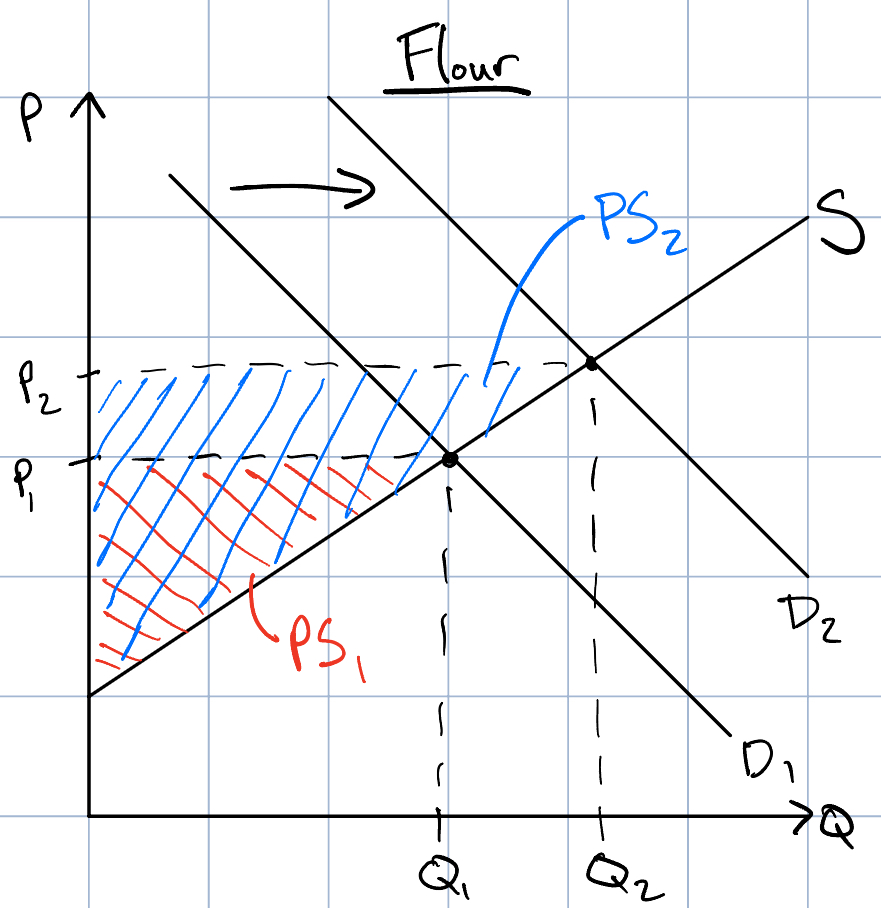
\includegraphics[width = 0.3\textwidth]{ch7_paa3_flour}
	\end{center}
	
\item

	\begin{enumerate}
	
	\item The schedule is below. The graph is in part (c).
		\begin{center}
		\begin{tabular}{c | c}
		$P$ & $Q_D$ \\
		\hline
		More than \$7 & 0 \\
		\$5 to \$7 & 1 \\
		\$3 to \$5 & 2 \\
		\$1 to \$3 & 3 \\
		Less than \$1 & 4
		\end{tabular}
		\end{center}
		
	\item He buys 2 bottles of water. Consumer surplus is \$4. See the graph in part (c) for the calculation.
	
	\item Quantity demanded increases to 3 bottles of water. Consumer surplus increases to \$9. 
	
		\begin{center}
		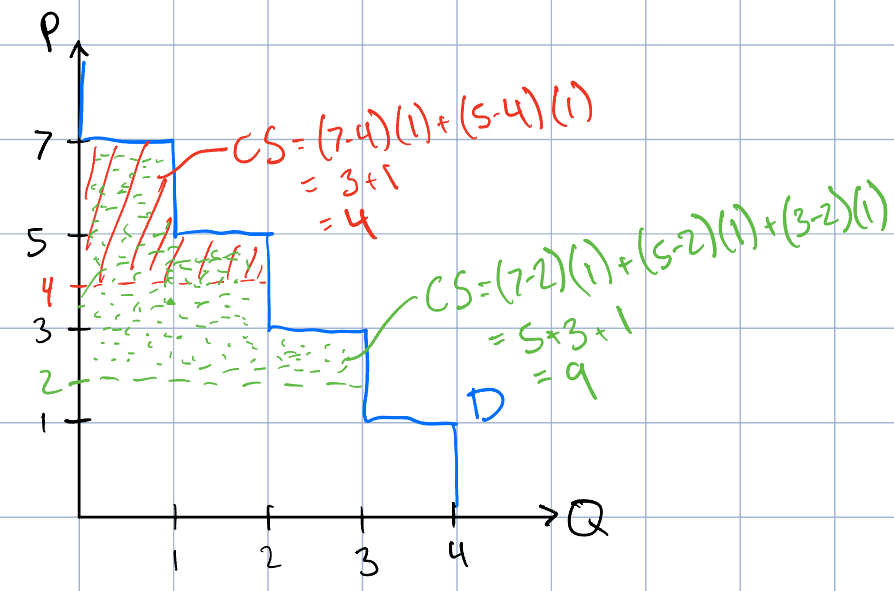
\includegraphics[width = 0.5\textwidth]{ch7_paa4}
		\end{center}
	
	\end{enumerate}
	
\item

	\begin{enumerate}
	
	\item The schedule is below. The graph is in part (c). 
		\begin{center}
		\begin{tabular}{c | c}
		$P$ & $Q_S$ \\
		\hline
		Less than \$1 & 0 \\
		\$1 to \$3 & 1 \\
		\$3 to \$5 & 2 \\
		\$5 to \$7 & 3 \\
		More than \$7 & 4
		\end{tabular}
		\end{center}
		
	\item He produces 2 bottles of water. His producer surplus is \$4. See the graph in part (c) for the calculation.
	
	\item Quantity supplied increases to 3 bottles of water. His producer surplus increases to \$9.
	
		\begin{center}
		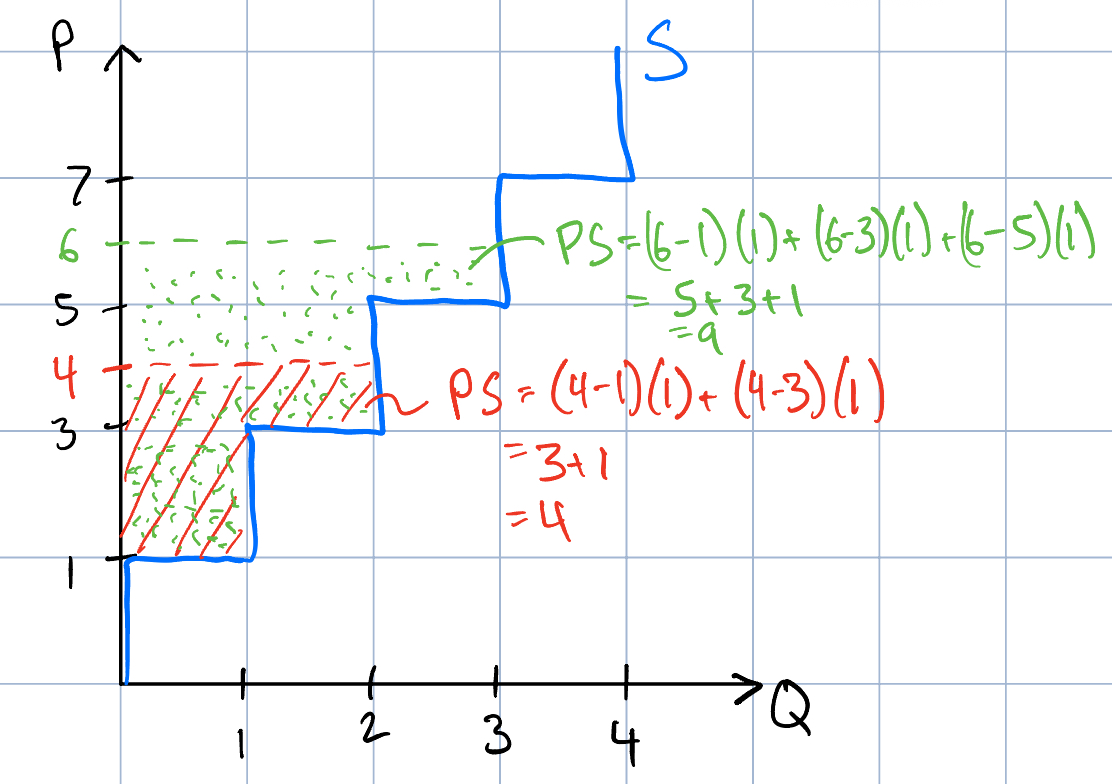
\includegraphics[width = 0.5\textwidth]{ch7_paa5}
		\end{center}
	
	\end{enumerate}
	
\item

	\begin{enumerate}
	
	\item Here I'm using the supply and demand schedules I made from 4.a. and 5.b.
		\begin{center}
		\begin{tabular}{c | c | c}
		$P$ & $Q_S$ & $Q_D$ \\
		\hline
		2 & 1 & 3 \\
		4 & 2 & 2 \\
		6 & 3 & 1 \\
		\end{tabular}
		\end{center}
		
		A price of \$4 brings supply and demand into equilibrium.
		
	\item From 4.b., we know consumer surplus is \$4. From 5.b., we know producer surplus is \$4. Total surplus is $TS = CS + PS = 4 + 4 = \$8.$
	
	\item Total surplus would decrease to $3 + 3 = 6$.
	
		\begin{center}
		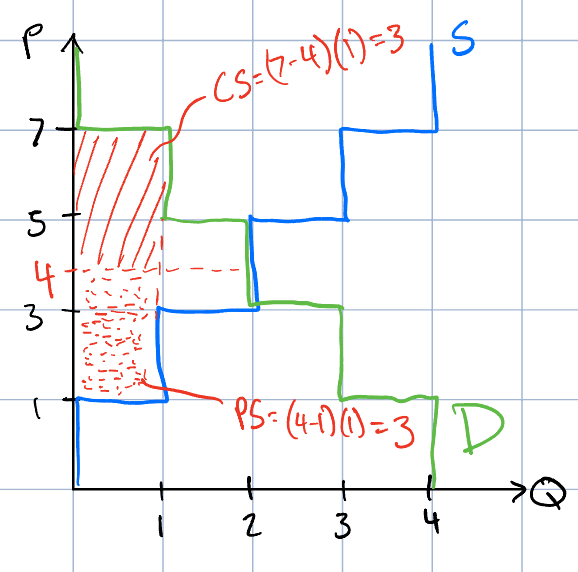
\includegraphics[width = 0.3\textwidth]{ch7_paa6c}
		\end{center} 
		
	\item Total surplus would decrease to $4 + 4 - 1 - 1 = 6$.
	
		\begin{center}
		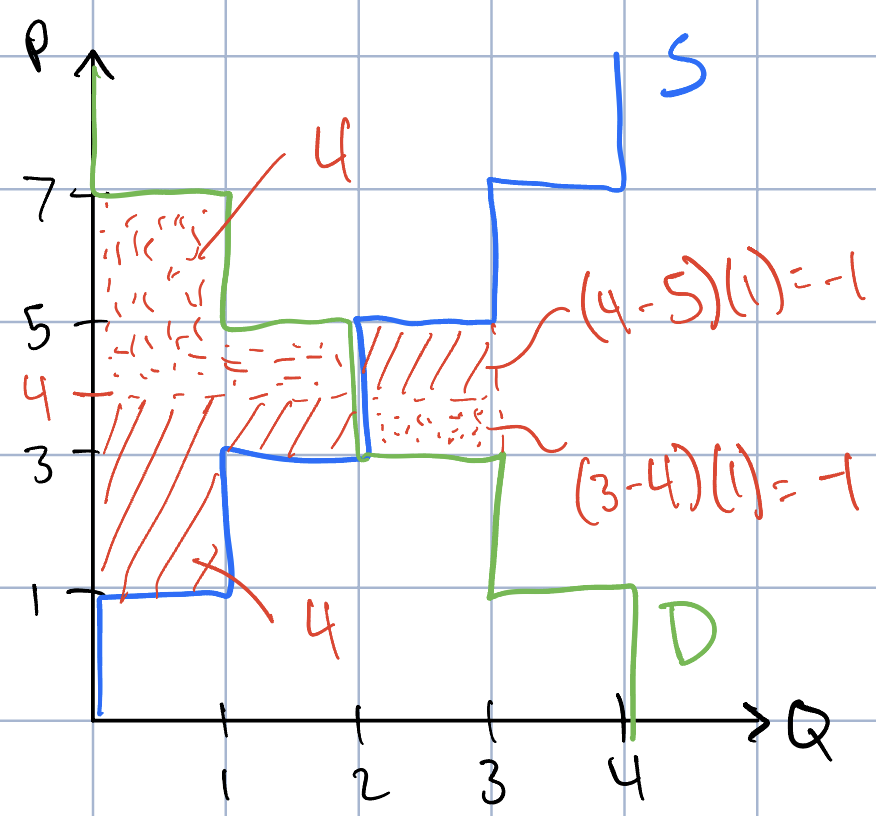
\includegraphics[width = 0.3\textwidth]{ch7_paa6d}
		\end{center}
	
	\end{enumerate}
	
\item

	\begin{enumerate}
	
	\item Supply shifts out in response to falling production costs, so price decreases, and quantity increases. See graph in (b).

	\item Both $CS$ and $PS$ increase.

		\begin{center}
		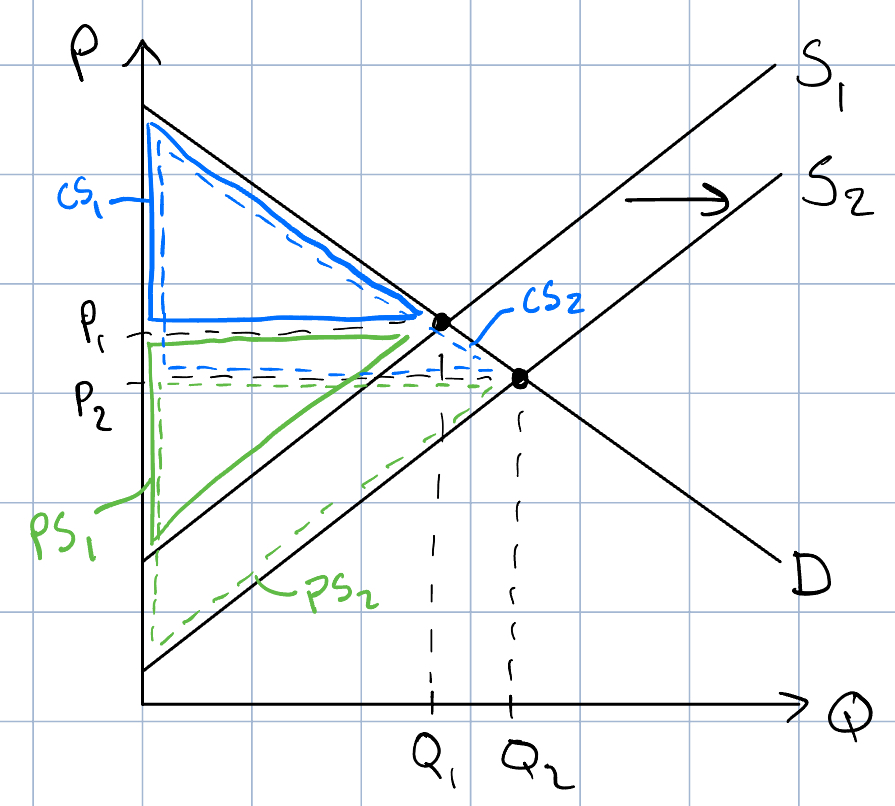
\includegraphics[width = 0.3\textwidth]{ch7_paa7ab}
		\end{center}
		
	\item Consumers would benefit most because consumer surplus increases more than producer surplus. 
	
		\begin{center}
		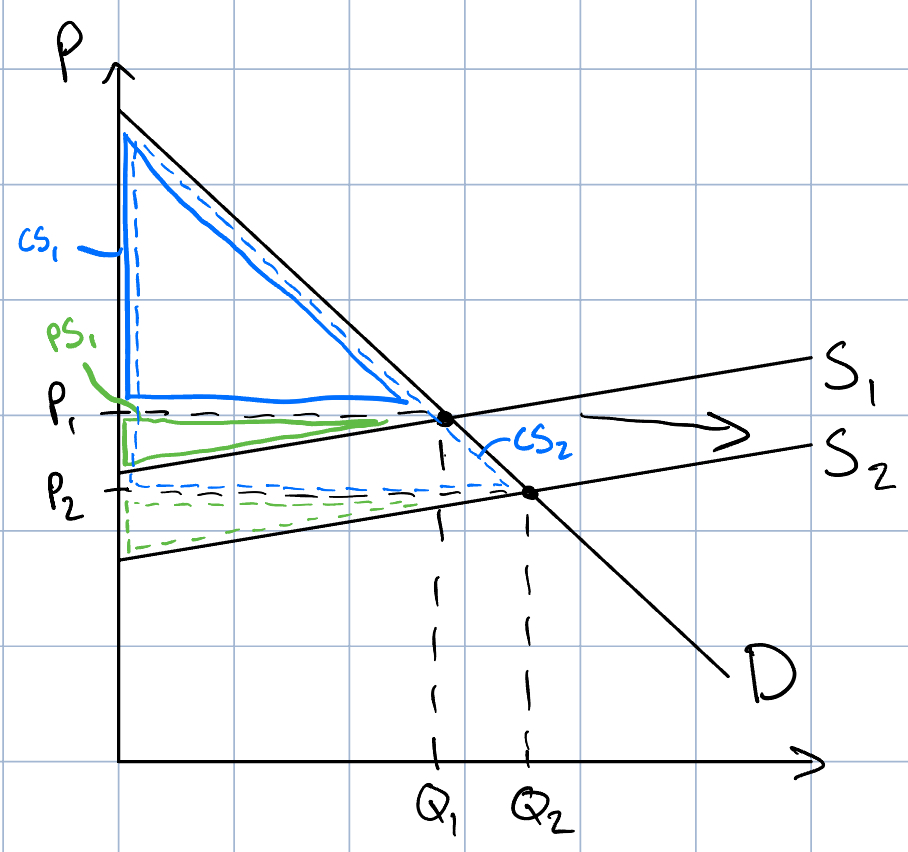
\includegraphics[width = 0.3\textwidth]{ch7_paa7c}
		\end{center}
	
	\end{enumerate}
	
\item There should be three haircuts given for a maximum of \$55 in total surplus. The first haircut should go to the person who values it the most and come from the firm that produces it for the lowest cost. That means Claire should buy a haircut from Firm D which generates $\$40 - \$10 = \$30$ of total surplus. The second haircut should go to the person who values it the second most and come from the firm that produces it for the second lowest cost. That means Gloria should buy a haircut from Firm B which generates $\$35 - \$15 = \$20$ of total surplus. The third haircut should go to the person who values it the third most and come from the firm that produces it for the third lowest cost. That means Phil should buy a haircut from Firm C which generates $\$25 - \$20 = \$5$ of total surplus. After that, the marginal buyer, Jay, values a haircut less than it costs the marginal seller, Firm B, to provide the service, so no more haircuts should happen. In this scenario, total surplus is $\$30 + \$20 + \$5 = \$55$. 

\item

	\begin{enumerate}
	
	\item The advancement in production technology will shift the supply curve out. That increases the equilibrium quantity and decreases the equilibrium price. As a result, consumer surplus and producer surplus both increase.
	
		\begin{center}
		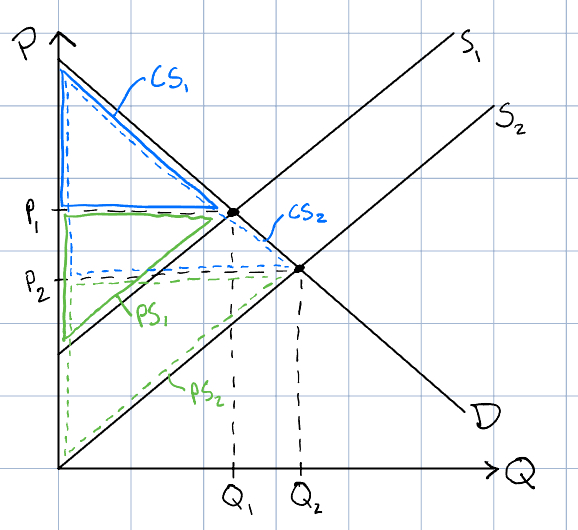
\includegraphics[width = 0.3\textwidth]{ch7_paa9a}
		\end{center}
	
	\item That makes typewriters and computers substitutes. The decreased price of computers shifted demand for typewriters left. That decreases the equilibrium quantity and price. As a result, consumer surplus and producer surplus both decrease. Typewriter producers should be sad about the technological advance because it decreases the value they accrue in the typewriter market.
	
	\begin{center}
	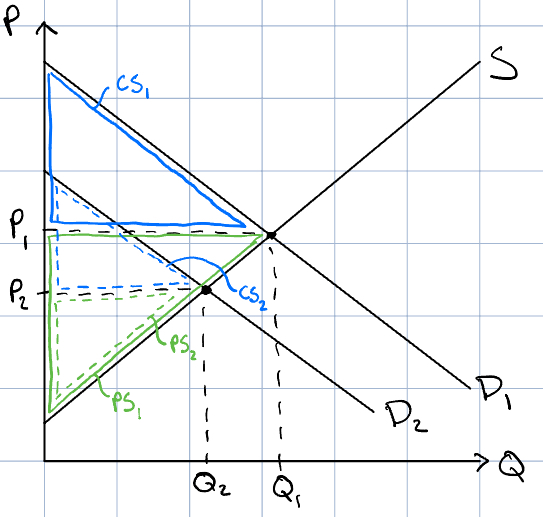
\includegraphics[width = 0.3\textwidth]{ch7_paa9b}
	\end{center}
	
	\item Computers and software are complements, so the decreased price of computers increases demand for software. That increases the equilibrium quantity and price of software. As a result, consumer surplus and producer surplus both increase. Software producers should be happy about the technological advance because it increases the value they accrue in the software market.
	
	\begin{center}
	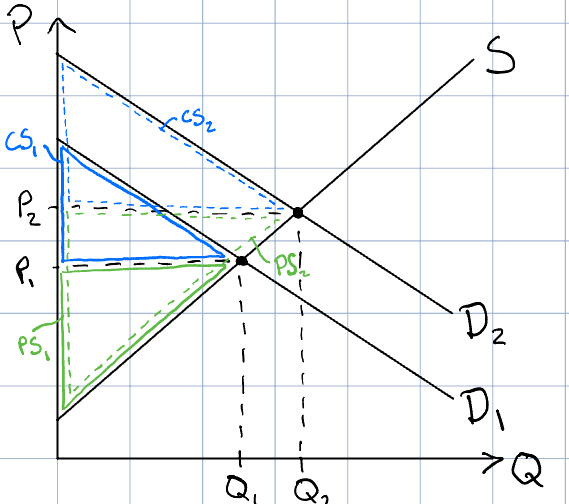
\includegraphics[width = 0.3\textwidth]{ch7_paa9c}
	\end{center} 
	
	\item It does. We see that software producers accrued a lot more surplus when computers became more widespread.
	
	\end{enumerate}
	
\item

	\begin{enumerate}
	
	\item Provider A: \$0 because each additional movie comes at no additional charge. \\
		Provider B: \$1 because each additional movie comes at a charge of \$1.
	
	\item The friend should buy until their willingness to pay for an additional movie equals the cost of an additional movie. \\
		
		\begin{center}
		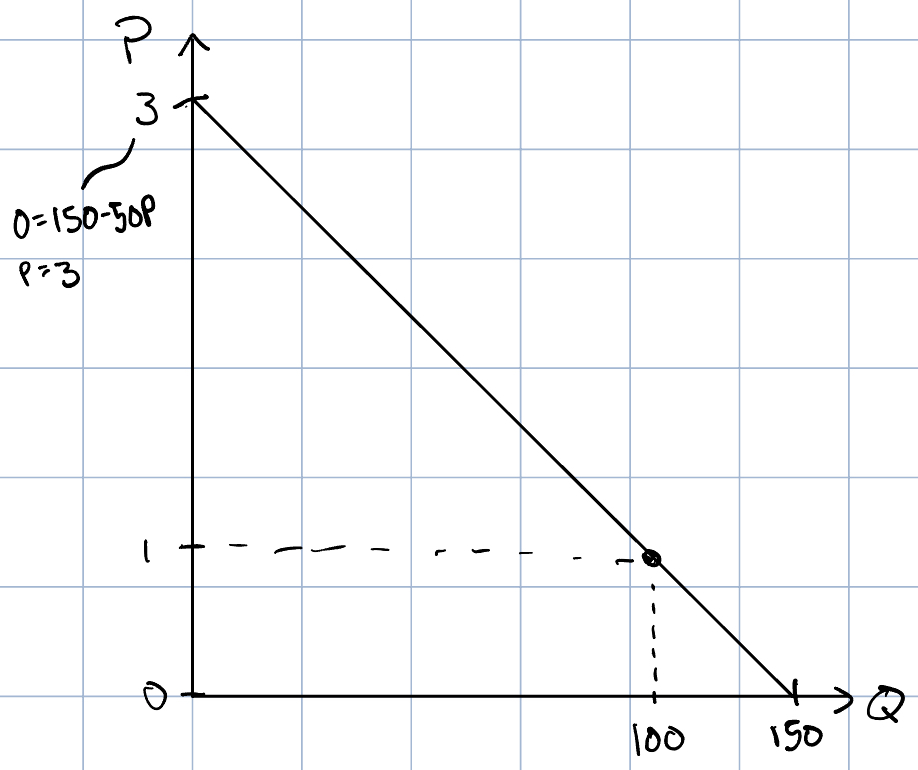
\includegraphics[width = 0.3\textwidth]{ch7_paa10}
		\end{center}
		
		Provider A: $Q_D = 150 - 50(0) = 150$\\ 
		Provider B: $Q_D = 150 - 50(1) = 100$
	
	\item She would pay Provider A the one time flat fee of \$120. She would pay Provider B \$1 per move, \$100.
	
	\item Provider A: \\
		Value accrued from movies = $\frac{1}{2}(3)(150) = \$225$ \\
		Total spent on movies = \$120 \\
		Consumer Surplus = $225 - 120 = \$105$ \\
		Provider B: \\
		Consumer Surplus = $\frac{1}{2}(3 - 1)(100) = \$100$
	
	\item I would recommend Provider A because they would get more consumer surplus from streaming through Provider A.
	
	\end{enumerate}

\end{enumerate}

\section*{Non-Textbook Questions}

\begin{enumerate}

\item

	\begin{enumerate}
	
	\item \begin{align*}
		10P - 40 &= 200 - 10P \\
		20P &= 240 \\
		P^* &= 12 \\
		Q^* &= 10(12) - 40 \\
		Q^* &= 80
		\end{align*}
		
	\item \phantom{x}
		\begin{center}
		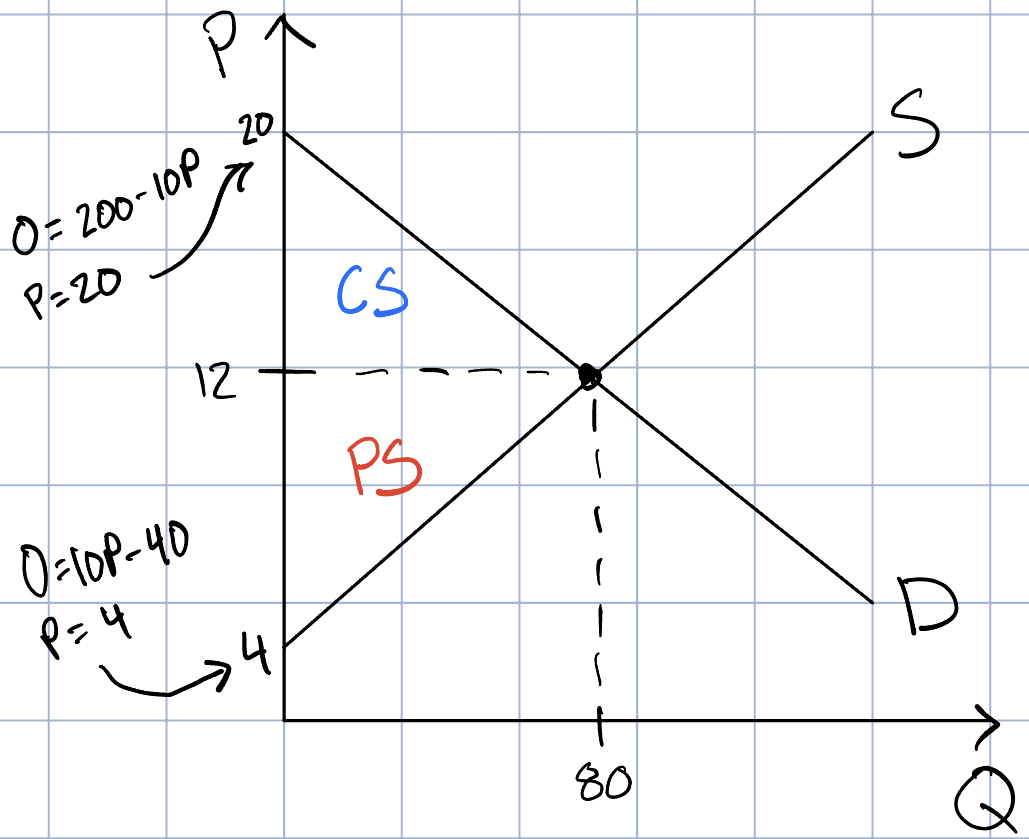
\includegraphics[width = 0.4\textwidth]{ch7_ntq1b}
		\end{center}
		\begin{align*}
		CS &= \frac{1}{2}(20 - 12)(80) \\
		&= 320 \\
		\end{align*}
		
	\item \begin{align*}
		PS &= \frac{1}{2}(12 - 4)(80) \\
		&= 320 
		\end{align*}
		
	\item \phantom{x}
		\begin{center}
		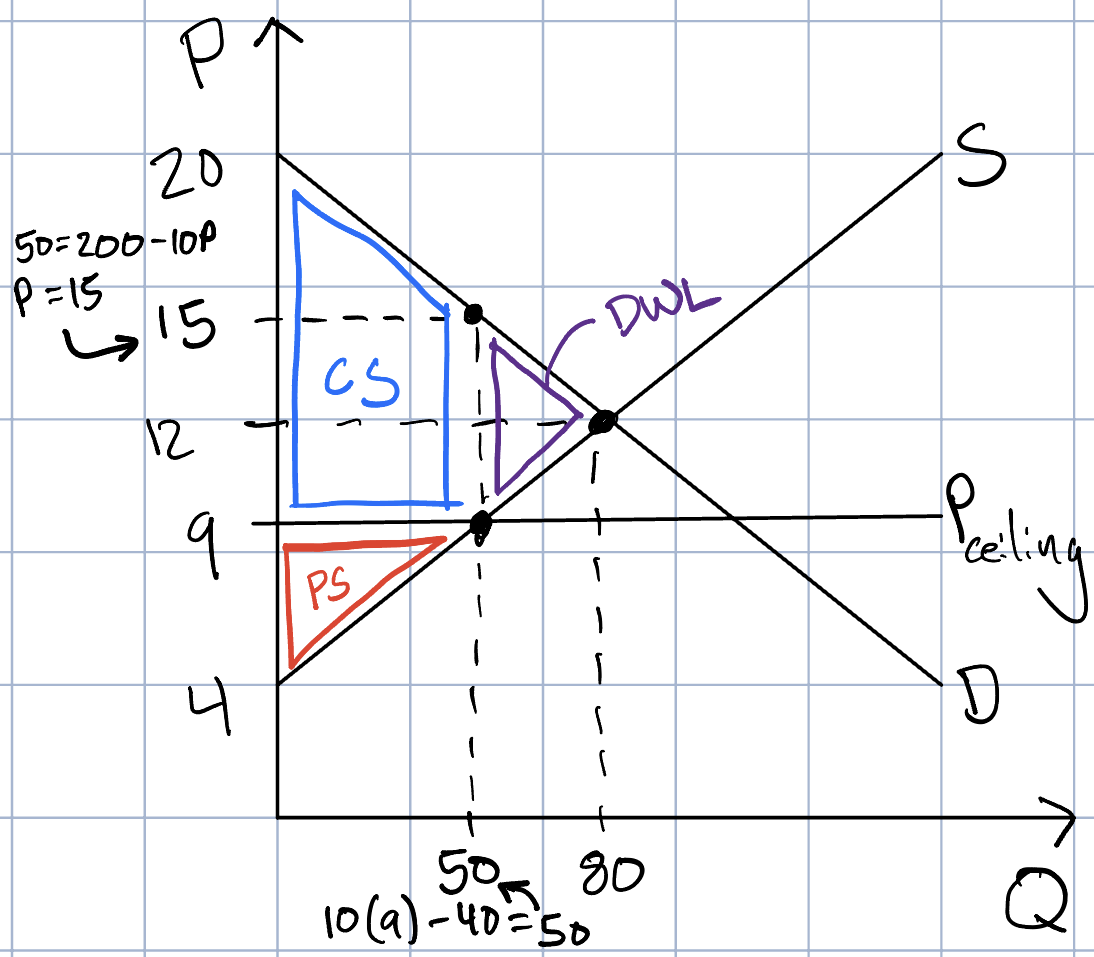
\includegraphics[width = 0.4\textwidth]{ch7_ntq1d}
		\end{center}
		\begin{align*}
		Q_{ceiling} &= 10(9) - 40 \\
		&= 50
		\end{align*}
		
	\item \begin{align*}
		CS &= \frac{1}{2}(20 - 15)(50) + (15 - 9)(50) \\
		&= 125 + 300 \\
		&= 425 \\
		PS &= \frac{1}{2}(9 - 4)(50) \\
		&= 125
		\end{align*}
		
	\item \begin{align*}
		DWL &= \frac{1}{2}(15 - 9)(80 - 50) \\
		&= 90
		\end{align*}
		
	\item The consumers who receive one of the 50 goods benefit because their price decreases relative to before. The consumers who would have bought at the market price but can't find a seller after the price ceiling lose. All of the producers lose -- both those who leave the market and those who remain in but receive a loewr price. 
	
	\end{enumerate}
	
\item

	\begin{enumerate}
	
	\item \begin{align*}
		60 - 10P &= 5P
		P^* &= 4
		\end{align*}
		The price ceiling isn't binding, so producer surplus won't change after the policy.
		
	\item \phantom{x}
		\begin{center}
		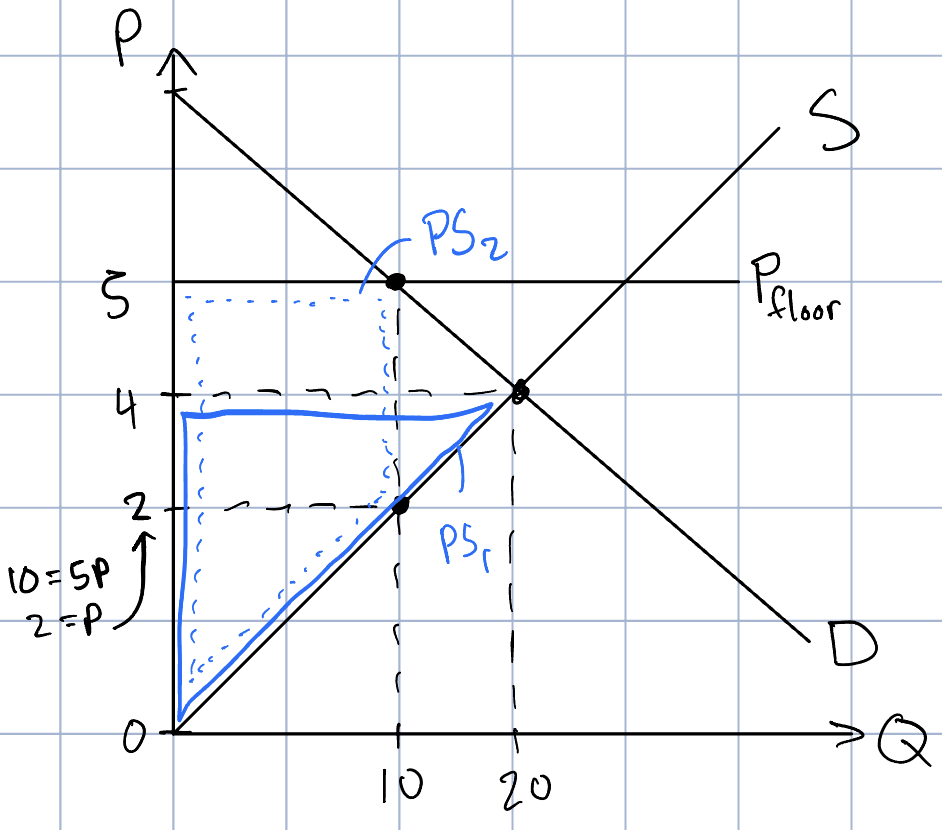
\includegraphics[width = 0.4\textwidth]{ch7_ntq2b}
		\end{center}
		 \begin{align*}
		Q^* &= 5(4) \\
		&= 20 \\
		PS_1 &= \frac{1}{2}(4)(20) \\
		&= 40 \\
		Q_{floor} &= 60 - 10(5) \\
		&= 10 \\
		PS_2 &= (5 - 2)(10) + \frac{1}{2}(2)(10) \\
		&= 40
		\end{align*}
		Producer surplus doesn't change after the policy.
		
	\item All consumers lose -- both those who exit the market and those who remain in but pay a higher price. The producers who can still find a buyer benefit because they receive a higher price. The producers who can no longer find a buyer lose.
	
	\end{enumerate}
	
\item

	\begin{enumerate}
	
	\item (I filled in the numbers for this graph as I worked through the problem. Initially, I just had the variables labeled.)
		\begin{center}
		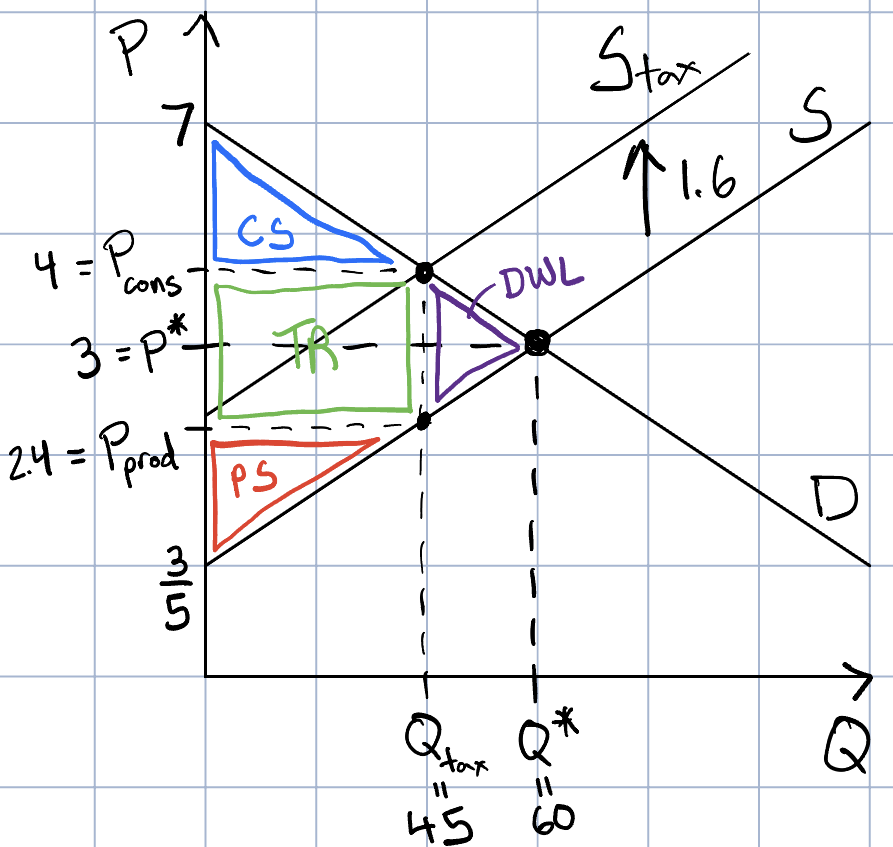
\includegraphics[width = 0.4\textwidth]{ch7_ntq3}
		\end{center}
		Inverse supply and demand:
		\begin{gather*}
		Q_D = 105 - 15P \\
		15P = 105 - Q_D \\
		P = 7 - \frac{1}{15}Q_D \\
		\\
		Q_S = 25P - 15 \\
		Q_S + 15 = 25P\\
		\frac{1}{25}Q_S + \frac{3}{5} = P
		\end{gather*}
		Inverse supply after the tax:
		\begin{gather*}
		P = \frac{1}{25}Q_S + \frac{3}{5} + 1.6 \\
		P = \frac{1}{25}Q_S + \frac{11}{5}
		\end{gather*}
		Quantity after the tax:
		\begin{align*}
		7 - \frac{1}{15}Q &= \frac{1}{25}Q + \frac{11}{5} \\
		\frac{24}{5} &= \frac{8}{75}Q \\
		45 &= Q_{tax}
		\end{align*}
		
	\item \begin{align*}
		P_{cons} &= 7 - \frac{1}{15}(45) \\
		&= 4 \\
		P_{prod} &= P_{cons} - 1.6 \\
		&= 2.4
		\end{align*}
		
	\item P-Intercepts of supply and demand:
		\begin{align*}
		0 &= 25P - 15 \\
		15 &= 25P \\
		\frac{3}{5} &= P \\
		\\
		0 &= 105 - 15P \\
		15P &= 105 \\
		P &= 7
		\end{align*}
		Surplus:
		\begin{align*}
		CS &= \frac{1}{2}(7 - 4)(45) \\
		&= \frac{135}{2} \\
		PS &= \frac{1}{2}\left(2.4 - \frac{3}{5}\right)(45) \\
		&= \frac{9}{10}(45) \\
		&= \frac{81}{2}
		\end{align*}
		
	\item \begin{align*}
		TR &= Q_{tax} \cdot t \\
		&= 45 \cdot 1.6 \\
		&= 72
		\end{align*}
		
	\item Pre-tax quantity:
		\begin{align*}
		105 - 15P &= 25P - 15 \\
		120 &= 40P \\
		3 &= P^* \\
		Q^* &= 25(3) - 15 \\
		&= 60
		\end{align*}
		Deadweight loss:
		\begin{align*}
		DWL &= \frac{1}{2}(4 - 2.4)(60 - 45) \\
		&= \frac{4}{5}(15) \\
		&= 12
		\end{align*}
	
	\end{enumerate}
	
\item

	\begin{enumerate}
	
	\item \begin{align*}
		CS &= \frac{1}{2}(3.65 - 2)(1.65 \text{ billion}) \\
		&= \$1.36125 \text{ billion} \\
		PS &= \frac{1}{2}(2 - 0.35)(1.65 \text{ billion}) \\
		&= \$1.36125 \text{ billion} \\
		TS &= CS + PS \\
		&= \$2.7225 \text{ billion}
		\end{align*}
		
	\item \begin{align*}
		CS &= \frac{1}{2}(3.65 - 2.05)(1.6 \text{ billion}) \\
		&= \$1.28 \text{ billion}
		\end{align*}
		
	\item \begin{align*}
		PS &= \frac{1}{2}(2.05 - 0.35)(1.7) \\
		&= \$1.445 \text{ billion}
		\end{align*}
		
	\item $\$2.05 \cdot 100 \text{ million} = 205 \text{ million} = 0.205 \text{ billion}$
	
	\item $TS = \$1.28 \text{ billion} + \$1.445 \text{ billion} - \$0.205 \text{ billion} = \$2.52 \text{ billion}$ 
	
		Total surplus is lower than the market equilibrium.
	
	\end{enumerate}

\end{enumerate}

\end{document}